\section{Ứng dụng mô hình ViHealthBERT xây dựng công cụ trích xuất danh sách triệu chứng từ miêu tả của bệnh nhân}
\subsection{Động lực}
Một số bệnh viện có thiết lập hệ thống tư vấn bệnh trực tuyến: người bệnh gửi thông tin cá nhân cùng miêu tả triệu chứng, bác sĩ sẽ đọc và đưa ra chẩn đoán dựa trên miêu tả của người bệnh. Tuy nhiên, đôi khi người bệnh đưa ra nhiều thông tin không liên quan, trong khi bác sĩ chỉ cần danh sách các triệu chứng cụ thể để biết được bệnh nhân đang gặp vấn đề gì.

Nhóm đề xuất sử dụng mô hình ViHealthBERT ứng dụng vào bài toán Medical Named Entity Recognition (Medical NER) Tiếng Việt để tự động trích xuất danh sách các triệu chứng từ miêu tả của bệnh nhân, giúp tăng hiệu suất làm việc ở các cơ sở khám chữa bệnh.

\subsection{Finetune mô hình ViHealthBERT cho tác vụ NER}
\subsubsection{Ngữ liệu huấn luyện}
Nhóm tiến hành finetune lại mô hình ViHealthBERT để giải quyết bài toán Medical NER Tiếng Việt trên tập ngữ liệu PhoNER\_COVID19\cite{truong-etal-2021-covid}. Bộ ngữ liệu có các thông số được trình bày trong bảng~\ref{tab:covid-ner-vietnamese-stats}
\begin{table}
\centering
\begin{tabular}{|l|l|l|l|l|l|}
\hline
\textbf{Entity type} & \textbf{Train} & \textbf{Valid} & \textbf{Test} & \textbf{All} \\
\hline
PATIENT\_ID & 3240 & 1276 & 2005 & 6521 \\
\hdashline
PERSON\_NAME & 349 & 188 & 318 & 855 \\
\hdashline
AGE & 682 & 361 & 582 & 1625 \\
\hdashline
GENDER & 542 & 277 & 462 & 1281 \\
\hdashline
OCCUPATION & 205 & 132 & 173 & 510 \\
\hdashline
LOCATION & 5398 & 2737 & 4441 & 12576 \\
\hdashline
ORGANIZATION & 1137 & 551 & 771 & 2459 \\
\hdashline
SYMPTOM \& DISEASE & 1439 & 766 & 1136 & 3341 \\
\hdashline
TRANSPORTATION & 226 & 87 & 193 & 506 \\
\hdashline
DATE & 2549 & 1103 & 1654 & 5306 \\
\hline
\# Entities in total & 15767 & 7478 & 11735 & 34984 \\
\hline
\# Sentences in total & 5027 & 2000 & 3000 & 10027 \\
\hline
\end{tabular}
\caption{Các thông số của tập ngữ liệu PhoNER\_COVID19\cite{truong-etal-2021-covid}}
\label{tab:covid-ner-vietnamese-stats}
\end{table}

\subsubsection{Thông số huấn luyện và kết quả}
Các thông số huấn luyện được mô tả trong bảng~\ref{tab:configurations}. Nhóm sử dụng các độ đo Precision, Recall và F1-Score để đánh giá kết quả huấn luyện. Với \textit{TP} là số lượng mẫu đúng được dự đoán đúng (True Positive), \textit{FP} là số lượng mẫu đúng nhưng được dự đoán sai (False Positive) và \textit{FN} là số lượng mẫu sai và được dự đoán sai (False Negative). Công thức tính Precision, Recall và F1-Score được định nghĩa như sau:
\begin{equation*}
\begin{aligned}
Precision (P) &= \frac{TP}{TP + FP} \\
Recall (R) &= \frac{TP}{TP + FN} \\
F1 &= \frac{2PR}{P + R}
\end{aligned}
\end{equation*}

Mô hình sau khi huấn luyện đạt được 95\% Precision, 94\% Recall và 95\% F1-Score khi đối chiếu với tập test của bộ ngữ liệu PhoNER\_COVID-19 đã nhắc ở phần trên. Kết quả huấn luyện của mô hình được mô tả trong bảng~\ref{tab:results-test}.
\begin{table}
\centering
\begin{tabular}{|l|c|}
\hline
\# epochs & 10 \\
\hline
batch size & 16 \\
\hline
seqlen & 70 \\
\hline
learning rate & 5e-5 \\
\hline
dropout rate & 0.1 \\
\hline
\end{tabular}
\caption{Thông số finetune mô hình ViHealthBERT cho tác vụ NER}
\label{tab:configurations}
\end{table}

\begin{table}
\centering
\begin{tabular}{|l|l|l|l|}
\hline
\textbf{label}        & \textbf{precision} & \textbf{recall} & \textbf{f1-score} \\ \hline
DATE                  & 0.9909             & 0.9921          & 0.9915            \\ \hdashline
SYMPTOM\_AND\_DISEASE & 0.9322             & 0.9040          & 0.9179            \\ \hdashline
NAME                  & 0.9073             & 0.9073          & 0.9073            \\ \hdashline
LOCATION              & 0.9529             & 0.9381          & 0.9454            \\ \hdashline
PATIENT\_ID           & 0.9857             & 0.9841          & 0.9849            \\ \hdashline
TRANSPORTATION        & 0.9442             & 0.9637          & 0.9538            \\ \hdashline
GENDER                & 1.0000             & 0.9776          & 0.9887            \\ \hdashline
ORGANIZATION          & 0.9064             & 0.9182          & 0.9123            \\ \hdashline
JOB                   & 0.8659             & 0.8208          & 0.8427            \\ \hdashline
AGE                   & 0.9803             & 0.9681          & 0.9741            \\ \hline
\textbf{micro avg}    & 0.9592             & 0.9497          & 0.9545            \\ \hline
\textbf{macro avg}    & 0.9592             & 0.9497          & 0.9544            \\ \hline
\end{tabular}
\caption{Kết quả finetune mô hình ViHealthBERT cho tác vụ NER trên tập test của bộ ngữ liệu PhoNER\_COVID-19}
\label{tab:results-test}
\end{table}

\subsection{Xây dựng ứng dụng}
Ứng dụng cần nhận biết và trích xuất các triệu chứng bệnh từ đầu vào là văn bản của người dùng. Do vậy, nhóm sẽ trích xuất các từ được gán nhãn \textit{SYMPTOM\_AND\_DISEASE} trong văn bản. Một ví dụ cho input (câu văn miêu tả triệu chứng) và output (danh sách các nhãn của câu) có thể thấy trong hình~\ref{fig:example-result}.
\begin{figure}
\centering
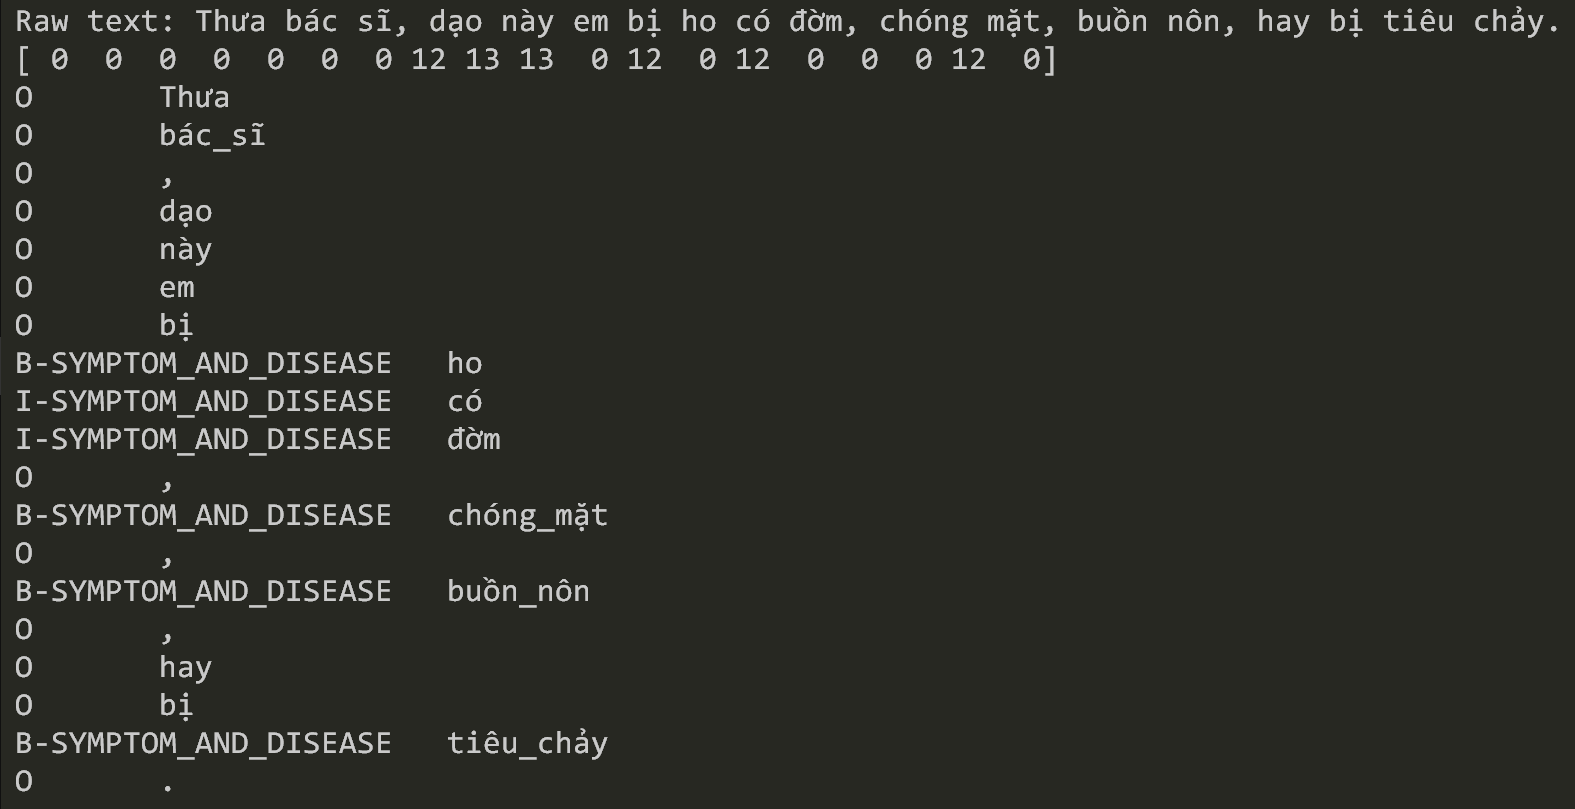
\includegraphics[scale=.5]{img/example-result.png}
\caption{Một ví dụ cho input (câu văn miêu tả triệu chứng) và output (danh sách các nhãn của câu)}
\label{fig:example-result}
\end{figure}

Thuật toán trích xuất các nhãn \textit{SYMPTOM\_AND\_DISEASE} được miêu tả trong Thuật toán \ref{alg:ner-retriever}

\begin{algorithm}
\caption{Thuật toán trích xuất các nhãn \textit{SYMPTOM\_AND\_DISEASE}}
\label{alg:ner-retriever}
\begin{algorithmic}
\Function {RetrieveSymptomsFromNERTags}{\textit{words}, \textit{labels}}
\State $list\_symptoms \gets \{\}$
\State $temp\_symptoms \gets \emptyset$
\State $n \gets |label|$
\For {$i \in [0, n - 1]$}
\If {$labels_i$ = B-SYMPTOM\_AND\_DISEASE}
\If {$temp\_symptoms \neq \emptyset$}
    \State Thêm $temp\_symptoms$ vào $list\_symptoms$
\EndIf
\State $temp\_symptoms \gets words_i$
\ElsIf {$labels_i$ = I-SYMPTOM\_AND\_DISEASE}
\State Thêm $words_i$ vào sau $temp\_symptoms$
\EndIf
\EndFor
\State\Return list\_symptoms
\EndFunction
\end{algorithmic}
\end{algorithm}

Với thuật toán này, nhóm tiến hành xây dựng ứng dụng web cho phép người dùng nhập vào một câu văn (đoạn văn). Dữ liệu được đưa vào mô hình ViHealthBERT đã được finetune để gán nhãn, sau đó bộ nhãn và câu đầu vào sẽ được đưa vào thuật toán đã nêu để trích ra danh sách các triệu chứng. Workflow của ứng dụng có thể được tóm tắt qua hình~\ref{fig:workflow}.
\begin{figure}
\centering
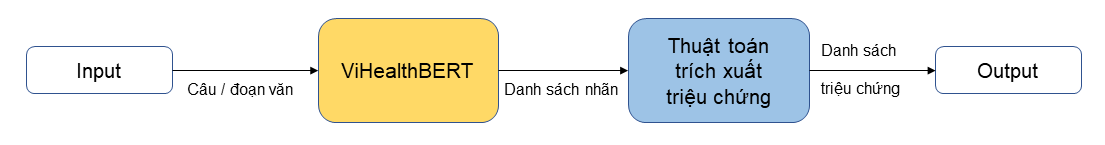
\includegraphics[scale=.6]{img/workflow.png}
\caption{Workflow ứng dụng trích xuất triệu chứng}
\label{fig:workflow}
\end{figure}
Nhóm sử dụng Flask framework để xây dựng ứng dụng web.
%% TODO: more description here
Nhóm xây dựng ứng dụng web bằng Flask framework (backend API) và Flutter (frontend).
